\chapter{Construction Tree Rules}

In this appendix, I have compiled in one place all of the rules for putting together construction trees for lambda terms. It does not correspond to any particular lecture, but is rather intended to be used as a reference material.

\section{Rules}
We first define $tree()$ as a function that takes a lambda expression to its construction tree. The simplest rule is for constants and variables. Let $x$ be a constant or variable. We then define
\begin{equation*}
  \hbox{tree}(x) := x
\end{equation*}

The tree of a term is
\begin{center}
  \begin{tikzpicture}[grow'=up]
    \Tree[.$(XY)$ [.{tree$(X)$} ] [.{tree$(Y)$} ] ];
  \end{tikzpicture}
\end{center}

Finally, we define tree$()$ of a lambda:
\begin{center}
  \begin{tikzpicture}[grow'=up]
    \Tree[.$\l zX$ [.$X$ ] ];
  \end{tikzpicture}
\end{center}